%!TEX root = ../../../../report.tex

\subsection{The electric actuators} % (fold)
\label{sub:electric_actuators}
In chapter \ref{cha:mathematical_model}, the necessary characteristics of the actuators have been calculated.
In this section, the resulting theoretical requirements are used to select the final motor $+$ gearbox combination utilized.
All the documentation regarding the control of the actuators software-wise is to be found in section \ref{sec:software}.

\subsubsection{Flat BLDC Maxon motors} % (fold)
\label{ssub:the_bldc_motors}
It must be mentioned at this point that the actuators and their interface were assumed at the beginning of the project to be a very hard constraint in the design from an economic point of view. 
This means that the conception of the robot structure has been influenced by this criteria towards the adaption of the final prototype characteristics (such as final size or mass) to the application range of the available motors at our disposal.
This fact has converted the design in an iterative process of optimization whose final result is a robot that matches the available actuators and not the other way around, as it should be in theory.
In the view of the this, the brushless DC motor $+$ gearbox present in the Locokit robot construction kit, introduced in \cite{locokit} are used in the RuBi prototype.

The flat motors model is 339260 from Maxon motor, whose datasheet can be found in \cite{maxon_motor}, and the planetary gearhead is the number 143976 in datasheet \cite{maxon_gear}.
The electromechanical constants of the motors, together with its nominal supply values or the output power and torque of both the motor and the gearbox can be found in these documents. 
However, the electronics of the motors are designed to constantly overdrive them at $24V$, which has been taken into account when calculating their output.
Furthermore, each motor counts three hall effect sensors able to provide accurate relative position measurements.
% subsubsection the_bldc_motors (end)


\subsubsection{BLDC motor boards} % (fold)
\label{ssub:bldc_motor_boards}
Each BLDC motor in the Locokit comes with a motor board able to control it, designed for 24V and 48W.
They consist of a 48MHz ARM7 processor for time critical control and motor commutation, as stated in \cite{locokit-electronics}, together with 4 general purpose I/O inputs for local sensor interface.
Furthermore, they have two available 8-pin interfaces for the motors, one of them with a standard flex connector used in most of Maxon flat motors.

% subsubsection bldc_motor_boards (end)

\subsubsection{Extension PCBs} % (fold)
\label{ssub:extension_pcbs}
Following the idea of reducing weight and inertias in the structure as explained in chapter \ref{cha:analysis}, it was decided to place all the electronics off-board.
In order to extend the existing motor flex interfaces, a simple extension PCB was manufactured for each device.
The boards have been designed with Eagle following the requirements of current when sizing the width of the paths given by the supplier.
The design lacks of vias which reduces the complexity and facilitates the manufacturing.
The board for the left leg, whose schematic can be seen in \ref{fig:pcb1}\footnote{For the right leg the schematic has been mirrored}, contains a flex connector, like the one originally found on the motor boards, mapped to an 8-pin Molex connector where the wiring to the BLDC board is connected.

\begin{figure}[ht]
	\centering
	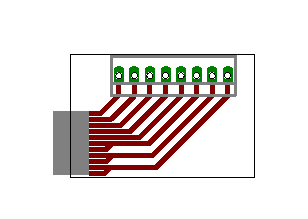
\includegraphics[width=0.5\textwidth]{figures/expansion_board.pdf}
	\caption{Left leg extension PCB schematic.}
	\label{fig:pcb1}
\end{figure}

% subsubsection extension_pcbs (end)


% subsection electric_actuators (end)
\subsection{Suitability of the motor model for the application} % (fold)
\label{sub:suitability_of_the_motor_model_for_the_application}
The algorithm designed to prove if the selected motor model fulfills the requirements of the application has been called Algorithm 1 and it is detailed in \ref{list:algorithm_1}.
The theoretical framework constructed in \ref{cha:mathematical_model} has been applied here to prove if the motors described above (without accounting on springs or indirect transmission) can be used to perform the vertical jumps described in \ref{sec:jumping_case}.
And if so, which height can be reached.

Algorithm 1:
\begin{enumerate}
\label{list:algorithm_1}
\item Manually set the values of $P_{3}(t_{0})$ and $P_{3}(t_{f})$ to use in equation \ref{eq:toe_trajectory}.
\item Compute the inverse kinematics model for the given trajectory equation. This yields as outputs $q_{j}(t)$, where j = 1,...,N being N = number of joints.
\item Compute forward kinematics to obtain $P_{j}(t)$.
\item Derive the two mentioned models and apply equation \ref{eq:angular_magnitudes} to obtain $\dot{P}_{j}$, $\ddot{P}_{j}$, $\omega_{j}$, $\omega_{j}$, $\dot{\omega}_{j}$,
\item Set $\Delta h$ and use the impulse equations \ref{eq:deltaV} and \ref{eq:impulse} to obtain a set of couple values of $(F_{i}, t_{i})$ as in Figure \ref{fig:f-t}.
\item For each couple until $(F_{min}, t_{max})$, obtained from \ref{eq:work}, compute the torques $\tau_{i,j}$ for each joint through \ref{eq:dynamics_eq1} and $\theta_{i,j}$ as in \ref{eq:joint_vel_2}\footnote{Eq. \ref{eq:joint_vel_2} introduced the assumption that the joint velocities are constant for simplicity}.
\item Compute the Torque/Speed curve for the motor + gearbox model as per equation \ref{eq:motor_curve}.
\item Plot the obtained pairs of values $(\dot{\theta}_{i,j}, \tau_{i,j})$ over the motor curve and analyze the results.
\end{enumerate}

\begin{equation}
\label{eq:joint_vel_2}
	\dot{\theta}_{i,j} =\frac{ \abs{ \theta_{j}(t_{f}) - \theta_{j}(t_{o}) } }{ t_{i} }
\end{equation}

\begin{equation}
\label{eq:motor_curve}
	\tau_{m} = \tau_{stall} - \omega_{m}\left(\frac{\tau_{stall}}{\omega_{n}}\right)
\end{equation}

\paragraph{Use case} % (fold)
\label{par:example_of_use}
As with any kind of DC motor, the goal is that the operation points lay under the torque/speed curve for a given application.
In this case, the operation point to study has been chosen to be the initial instant of the launch phase during the jump, given by $t_{0}=0s$, because it has been assumed to be the most requiring one of the whole jump cycle.
The input data for the test conducted with the algorithm can be seen in \ref{eq:input_a1}.

\begin{equation*}
\label{eq:input_a1}
\begin{aligned}[c]
P_{3}(t_{0}) &= \left[\!
				    \begin{array}{c}
				      0 \\
				      0.3508 \\
				      -\frac{\pi}{2}
				    \end{array}
				  \!\right]
\end{aligned}
\qquad
\begin{aligned}[c]
P_{3}(t_{f}) &= \left[\!
				    \begin{array}{c}
				      0 \\
				      L \\
				      0
				    \end{array}
				  \!\right]
\end{aligned}
\qquad
\begin{aligned}[c]
\Delta h &= 0.05 \\
\end{aligned}
\end{equation*}

The results can be seen in Figure \ref{fig:alg1_results} for a jumping leg.
It can be seen that, for the obtained $(\theta_{i,j}, \tau_{i,j})$ values for the given $\Delta h$, the closer they get to the theoretical $(F_{min}, t_{max})$, the more the application points approach the lower-left corner of the graph.
The aimed situation here is that in which the application points for the three motors lay under the motor curve, which occurs for values next to the couple $(4.1191N, 0.1700s)$

\begin{figure}[htb]
	\centering
	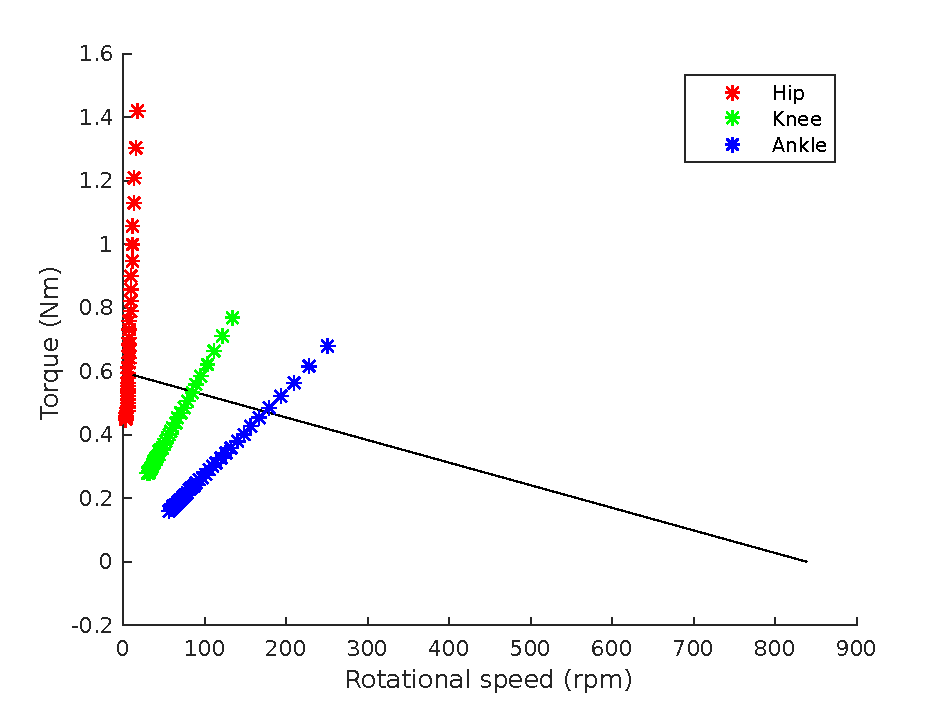
\includegraphics[width=0.9\textwidth]{figures/algorithm1.pdf}
	\caption{Results of Algorithm 1 for the given inputs (not all the $(\theta_{i,j}, \tau_{i,j})$ pairs are plotted).}
	\label{fig:alg1_results}
\end{figure}

\paragraph{The transmission on the hips} % (fold)
\label{par:the_hip_joint_gears}
The results from the presented algorithm helped notice that the presented motor model would not be able to accomplish the requirements of the application on the hip joints, due to its, in general, lower velocity and higher torque values.
Thus, the algorithm was used to approximate the required ratio of the gear system described in \ref{sub:gears}, used to adequate its output to the task.
The final ratio implemented and used for the results in \ref{fig:alg1_results} is $w=2$. 
However, it was calculated for the geometrical and inertial parameters of a different iteration than the last one, resulting in a non-optimal value for the final robot.
A repetition of the process yielded an optimal gear ratio of $w=1.2$, for which the best application points of the three motors would be closer to the motor line.

% paragraph the_hip_joint_gears (end)

The presented method does not aim at providing exact results since its based in several assumptions and simplifications from its basis.
It was conceived due to the necessity of assessing the utility of the existing actuators to the designed application.
Ideally, its results would have been tested by comparing them to the real data collected from the experimentation with the final prototype. 
However, the delay in some essential components of the robot prevented from testing and improving the model used for the algorithm, together with its validity.

% paragraph example_of_use (end)




% subsection suitability_of_the_motor_model_for_the_application (end)